% Opsætter KU Tex
%%%%%%%%%%%%%%%%%%%%%%%%%%%%%%%%%%%%%%%%%%%%%%%%%%%%%%%%%%%%%%%%%%%%%%%%%%%%%%%%
\documentclass[14pt]{article}
\usepackage[a4paper, hmargin={2.8cm, 2.8cm}, vmargin={2.5cm, 2.5cm}]{geometry}
\usepackage{eso-pic}  % \AddToShipoutPicture
\usepackage{graphicx} % \includegraphics
%%%%%%%%%%%%%%%%%%%%%%%%%%%%%%%%%%%%%%%%%%%%%%%%%%%%%%%%%%%%%%%%%%%%%%%%%%%%%%%%
\usepackage{float}

\usepackage{subfig}
\usepackage{url}
\usepackage{xcolor}
\usepackage{listings}

% Pakker til skrifttyper, tekst osv.
%%%%%%%%%%%%%%%%%%%%%%%%%%%%%%%%%%%%%%%%%%%%%%%%%%%%%%%%%%%%%%%%%%%%%%%%%%%%%%%%
    \usepackage[utf8]{inputenc} % Implementere Unicode
    \usepackage[T1]{fontenc}    % Unicode skrifttype, fx. é skrives som 1 tegn
   \usepackage[english]{babel} % Engelsk Ordbog
  % \usepackage[danish]{babel}  % Dansk Ordbog
    \usepackage{microtype}      % Forbedre linjeombrydningen
    \usepackage{libertine}      % Skrifttype
    \usepackage[scaled=0.83]{inconsolata} % Skrifttype til kode til kode
%%%%%%%%%%%%%%%%%%%%%%%%%%%%%%%%%%%%%%%%%%%%%%%%%%%%%%%%%%%%%%%%%%%%%%%%%%%%%%%%

% Pakker til matematik og kode.
%%%%%%%%%%%%%%%%%%%%%%%%%%%%%%%%%%%%%%%%%%%%%%%%%%%%%%%%%%%%%%%%%%%%%%%%%%%%%%%%
    \usepackage{mathtools}       % Udvidelse til amsmath pakken
   \usepackage{algpseudocode}   % pseudocode til algoritmer
    \usepackage{algorithm}       % Pakke til algoritmer
    \usepackage{amsthm}          % Pakke til Theroms
%%%%%%%%%%%%%%%%%%%%%%%%%%%%%%%%%%%%%%%%%%%%%%%%%%%%%%%%%%%%%%%%%%%%%%%%%%%%%%%%

% Pakker til layout.
%%%%%%%%%%%%%%%%%%%%%%%%%%%%%%%%%%%%%%%%%%%%%%%%%%%%%%%%%%%%%%%%%%%%%%%%%%%%%%%%
    \usepackage{fancyhdr}        % Gør det muligt at bruge sidehoveder
    \usepackage{graphicx}        % Mulighed for bl.a. \includegraphics
    \usepackage{parskip}         % Første paragraf i afsnit indrykkes ikke
    \usepackage{listings}        % Pakke til at indsætte kode
    \usepackage{enumitem}        % Gør det muligt at tilpasse lister
    \usepackage{titlesec}        % Tilpassing af afstand mellem sektioner
    \usepackage[lastpage,user]{zref} % Side x af y
%%%%%%%%%%%%%%%%%%%%%%%%%%%%%%%%%%%%%%%%%%%%%%%%%%%%%%%%%%%%%%%%%%%%%%%%%%%%%%%%

% Implementerer en række makroer og de pakker der er importeret
%%%%%%%%%%%%%%%%%%%%%%%%%%%%%%%%%%%%%%%%%%%%%%%%%%%%%%%%%%%%%%%%%%%%%%%%%%%%%%%%
    \pagestyle{fancy}                        % Implementerer sidehoved
    \lhead{Espergærde Gymnasium} % Venstre sidehoved
    \rhead{Machine Learning opgave}      % Højre sidehoved
    \cfoot{\thepage\ of \zpageref{LastPage}} % Side x af y
    \newtheorem*{prp}{Propostion}            % Skaber nyt theorem
    \setlist{nolistsep}              % Formindsker mellemrum mellem listepunkter

    % Definitioner af farver
    %%%%%%%%%%%%%%%%%%%%%%%%%%%%%%%%%%%%%%%%%%%%%%%%%%%%%%%%%%%%%%%%%%%%%%%%%%%%
        \definecolor{KURed1}{RGB}{144,26,30}    % Official KU Red 1
        \definecolor{KURed2}{RGB}{199,36,41}    % Unofficial KU Red
        \definecolor{KUGray1}{RGB}{102,102,102} % Official KU Gray 1
        \definecolor{KUGray2}{RGB}{133,133,133} % Official KU Gray 2
        \definecolor{KUGray3}{RGB}{163,163,163} % Official KU Gray 3
        \definecolor{KUGray4}{RGB}{194,194,194} % Official KU Gray 4
        \definecolor{KUGray5}{RGB}{224,224,224} % Official KU Gray 5
    %%%%%%%%%%%%%%%%%%%%%%%%%%%%%%%%%%%%%%%%%%%%%%%%%%%%%%%%%%%%%%%%%%%%%%%%%%%%

    % Mindsker afstanden mellem sektioner
    %%%%%%%%%%%%%%%%%%%%%%%%%%%%%%%%%%%%%%%%%%%%%%%%%%%%%%%%%%%%%%%%%%%%%%%%%%%%
        \titlespacing\section{0pt}{12pt plus 4pt minus 2pt}
                                  {0pt plus 1pt minus 3pt}
        \titlespacing\subsection{0pt}{12pt plus 4pt minus 2pt}
                                  {0pt plus 1pt minus 3pt}
        \titlespacing\subsubsection{0pt}{12pt plus 4pt minus 2pt}
                                  {0pt plus 1pt minus 3pt}
    %%%%%%%%%%%%%%%%%%%%%%%%%%%%%%%%%%%%%%%%%%%%%%%%%%%%%%%%%%%%%%%%%%%%%%%%%%%%

    % Laver titel
    %%%%%%%%%%%%%%%%%%%%%%%%%%%%%%%%%%%%%%%%%%%%%%%%%%%%%%%%%%%%%%%%%%%%%%%%%%%%
    \title{
      \vspace{13em}
      \huge{Espergærde Gymnasium\\}
      \Huge{Opgave i Machine Learning}
    }

    \author{
        \Large{
            Benjamin Rotendahl --- Benjamin@Rotendahl.dk
        }
    }
    \date{
        \vspace{22em}
        \today \\
    }

    \lstset{
      language=C,                     % choose the language of the code
      numbers=left,                   % where to put the line-numbers
      stepnumber=1,                   % the step between two line-numbers.
      numbersep=5pt,                  % distance from line-numbers to the code
      backgroundcolor=\color{white},  % choose the background color.
      showspaces=false,               % show spaces adding particular underscore
      showstringspaces=false,         % underline spaces within strings
      showtabs=false,                 % show tabs within strings
      tabsize=4,                      % sets default tabsize to 4 spaces
      captionpos=b,                   % sets the caption-position to bottom
      breaklines=true,                % sets automatic line breaking
      breakatwhitespace=true,         % breaks should only happen at whitespace
      title=\lstname,                 % show the filename of files included
    }
    %%%%%%%%%%%%%%%%%%%%%%%%%%%%%%%%%%%%%%%%%%%%%%%%%%%%%%%%%%%%%%%%%%%%%%%%%%%%
%%%%%%%%%%%%%%%%%%%%%%%%%%%%%%%%%%%%%%%%%%%%%%%%%%%%%%%%%%%%%%%%%%%%%%%%%%%%%%%%
%%%%%%%%%%%%%%%%%%%%      Her starter dokumentet    %%%%%%%%%%%%%%%%%%%%%%%%%%%%
\begin{document}


    %% Change `ku-farve` to `nat-farve` to use SCIENCE's old colors or
    %% `natbio-farve` to use SCIENCE's new colors and logo.
    \AddToShipoutPicture*{\put(0,0){\includegraphics*[viewport=0 0 700 600]
    {include/ku-farve}}}
    \AddToShipoutPicture*{\put(0,602){\includegraphics*[viewport=0 600 700 1600]
    {include/natbio-farve}}}

    %% Change `ku-en` to `nat-en` to use the `Faculty of Science` header
    \AddToShipoutPicture*{\put(0,0){\includegraphics*{include/nat-en}}}
    \clearpage

%Disse linjer skaber forside, evt indholdsfortegnelse, og sætter sidetal
%%%%%%%%%%%%%%%%%%%%%%%%%%%%%%%%%%%%%%%%%%%%%%%%%%%%%%%%%%%%%%%%%%%%%%%%%%%%%
    \maketitle{}              % Forside
    \thispagestyle{empty}   % Fjerner sidetal forside
    \newpage                % Første rigtige side
%%%%%%%%%%%%%%%%%%%%%%%%%%%%%%%%%%%%%%%%%%%%%%%%%%%%%%%%%%%%%%%%%%%%%%%%%%%%%

\section*{Introduktion til opgaven}
Denne opgave er en videreudvidelse til det machine learning i lærte den 1/2.
Målet med opgaven er at implementere en ``Supervised Learning'' algoritme der
kan kende forskel på kræftpatienter.

Data'en til opgaven er en større del af data'en fra perceptron algoritmen.
Hvert data punkt består af et sæt $(x, y)$ hvor $x$ er en vektor i $10$
dimensioner og $y$ er et ``label'', der enten er  $1$ for at indikere en
godartet svulst eller $-1$ for en ondartet. Formatet for $x$ er:
\begin{center}
    \begin{tabular}{| c | r |}
        \hline
        Threshold                & 1           \\ \hline
        Clump Thickness          & 7           \\ \hline
        Uniformity of Cell Size  & 1           \\ \hline
        Uniformity of Cell Shape & 4           \\ \hline
        Epithelial Cell Size     & 2           \\ \hline
        Bare Nuclei              & 3           \\ \hline
        Bland Chromatin          & 8           \\ \hline
        Normal Nucleoli          & 10          \\ \hline
        Mitoses                  & 3           \\ \hline
    \end{tabular}
\end{center}

Målet med opgaven er at lave en funktion der kan tage en patient som input og
giver et label som output.


\section*{Introduktion til algoritmen}
Algoritmen vi skal bruge er den såkaldte \emph{K Nearest Neighbor}(NN), vi
benytter den i varianten hvor $k=3$. Navnet til algoritmen skyldes at den
benytter ideen om ``naboskab/enshed'' til at forudse hvilke labels den skal
tilskrive data punkter. Uformelt kan ideen opsummeres med følgende scenarie:
\begin{itemize}
    \item Du har en veninde der hedder Anna og en ven der hedder Anders.
    \item Du kan godt lide samme musik, film, mad osv. som Anna kan lide.
    \item Anders kan normalt bedst lide ting du ikke kan.
    \item Anders og Anna har været på et nyt sted og spise.
    \item Anna synes stedet var godt, Anders kunne ikke lide det.
\end{itemize}
Givet de fem stykker information præsenteret ovenfor, gætter du på du ville
synes det nye sted eller ej? Siden at du generelt har meget tilfælles med Anna,
ville det være mest rimeligt at gætte på ja.

NN benytter samme tanke gang, da vi arbejde med vektorer der ikke har nogen
mening skal vi bruge en måde at måle naboskab. Ser vi på vektorerne som værende
repræsenteret i det Euklidiske rum kan afstandsformlen bruges til at måle hvor
``ens'' de er.
Afstandsformlen er defineret som:
$$
    d = \sqrt{\sum_{i=0}^{i=d} (u_i - v_i)^2}
$$
For at gøre formlen simplere dropper vi kvadratroden, dette kan vi gøre da vi
er ligeglade med den faktiske afstand mellem punkter og kun interessere os for
forholdet mellem. Det er lige meget om vi har $|AB| = 5, |AC| = 4$ eller
$|AB| = 25, |AC| = 16$, da vi stadig kan se at afstanden mellem $|AC|$ er
kortets. Derfor bruger vi følgende formel der er mere overskuelig og effektiv
da kvadratroden er en ``dyr'' operation for computere.
$$
    d = \sum_{i=0}^{i=d} (u_i - v_i)^2
$$


\newpage
    \begin{figure}[ht]
        \centering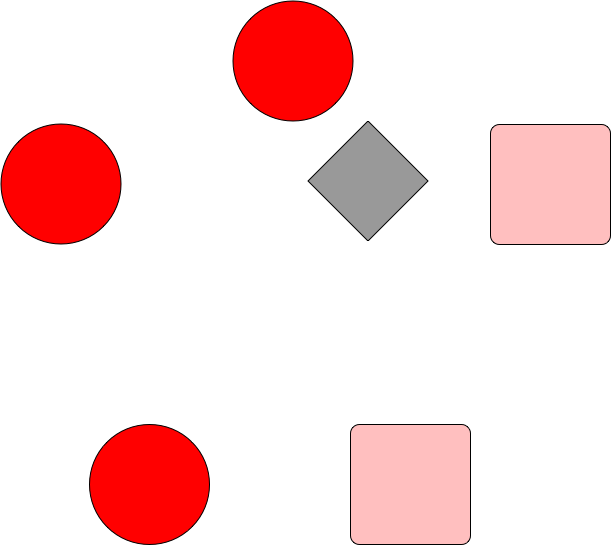
\includegraphics[scale=0.3]{include/3NN.png}
        \caption{Eksempel på punkter i rummet}
    \end{figure}
    Givet overstående figur skal vi bestemme om den grå diamant en cirkel
    eller en firkant. Det første vi gør er at bestemme afstanden til alle
    punkterne for at se hvilke tre den er tættest på. Vi ser at den er tættest
    på 2 cirkler og en firkant. Eftersom at det er 2 mod 1, konkluderer vi at
    det er mest sandsynligt at det er en cirkel.

    $k$'et i \emph{K Nearest Neighbor} afgør hvor mange nabo'er vi sammenligner
    med. Alt efter hvilket $k$ vi vælger havde vi fået et forskelliget svar.
    Valget afhænger af datasættet og er noget man kan prøve sig frem med.

    Algoritmen kan opsummeres i følgende trin, givet punktet $p$ og data sættet
    $D = [(x_1,y_1),(x_2,y_2),\dots (x_n,y_n)$ skal følgende trin udføres:
    \begin{enumerate}
        \item Beregn afstanden fra $p$ til alle punkter $x$.
        \item Find de $3$ punkter hvor afstanden var mindst.
        \item Se om der er flest naboer med $-1$ eller $1$.
        \item Meld flertallets markering tilbage.
    \end{enumerate}




\section*{Introduktion til koden}
Sammen med denne pdf er der udleveret en fil ved navn \emph{opgave.php},
i denne fil er der 5 funktioner der skal implementeres før algoritmen virker.
Kan du ikke køre \emph{php} på din maskine kan du åbne koden i f.eks notepad
og kopiere den ind på f.eks http://www.writephponline.com

Nedenfor præsenteres de fem funktioner og deres indgangs og udgangsbetingelser
sammen med nogle tips.

I koden kan variablen \emph{\$data} bruges til at tilgå data'en.
\begin{itemize}
    \item \emph{\$data[i]} Giver det datapar på formen $(y,x)$ der står på
    plads $i$
    \item \emph{\$data[i][0]} Giver markeringen for det $i$´te data par altså
    $y_i$
    \item \emph{\$data[i][1]} Giver vektoren for det $i$´te data par altså
    $x_i$
\end{itemize}

    \begin{description}
        \item[dist --- Afstandsfunktionen]
        Denne funktion modtager to vektorer og skal bruge afstandsformlen til at
        returnere hvor langt der er mellem dem.
        Altså givet de to vektorer
        $u = \left(\begin{array}{c} 9\\ 2\\ -1\\\end{array} \right)$
        og
        $v = \left(\begin{array}{c} 3\\ 5\\ 7\\\end{array} \right)$
        Skal den returnere:
        $$
            (9-3)^2 + (2-5)^2 + (-1-7)^2 = 109
        $$
        \textbf{Hint : Lav en værdi der først regner $(9-3)^2$ ud og så lægger de andre oven i}\\

        \item[guessLabel --- Gæt label]
        Denne funktion modtager en liste på formen $[-1, 1, -1]$.
        Den skal så tælle om der er flest $-1$ eller $1$ og returnere den der er
        flest af.
        \textbf{Hint : Det kan gøres med et regnestykke og en if statement}\\

        \newpage

        \item[sortClose --- Sorter de nærmeste]
        Vi ønsker at holde styr på en ``afstandsvektor'' der fortæller os hvilke
        3 punkter der lige nu er tættest på vores nye punkt. Denne funktion
        modtager data på formen $[[2,109], [1,152], [2,293]]$, hvor det første tal
        i parret $[2,109]$ står for hvilken plads i \emph{data} den har, og
        det andet tal er afstanden til $p$
        Målet er at returnere en liste hvor det altid er den med højest afstand
        der står først. Så svaret er:
        $$
            [[2,293], [2,109], [1,152]]
        $$
        Det smarte ved denne funktion er at vi nemmere kan holde styr på de tre
        der er tættest da det altid vil være den første vi skal udskifte hvis en
        var lavere.
        \textbf{Hint : Lav en ny tom liste, find det største element og placer det
        først}\\


        \item[getClosest --- Find de nærmeste]
        Funktionen skal lede hele \emph{\$data} igennem, finde de punkter der
        er nærmest og returnere en liste  på formen
        $[[i_1, d_1],[i_2, d_2], [i_3, d_3]]$
        Hvor $i$ punktets plads, og $d$ er dens afstand.
        \textbf{Hint : Start med at gæt på at de $3$ første punkter er nærmest og
        brug \emph{sortClose} til at få nye element ind i listen. }\\


        \item[NearestNeighbours --- 3NN]
        Kalder alle de overstående funktioner og er bindeled mellem dem.

    \end{description}
\end{document}
